\documentclass[9pt]{beamer}

% Fill in variables below %
% ++++++++++++++++++++++++++++++++++++++++++++++++++++++++++++++++++++++++ %
\newcommand{\thesemester}{Spring 2012}
\newcommand{\themidterm}{CS 61A Midterm 2 Review}
\newcommand{\theauthors}{Dan Wang, Chris Giola, and Jon Kotker}
\newcommand{\theorganization}{Eta Kappa Nu, Mu Chapter \\
University of California, Berkeley}
\newcommand{\thedate}{3 March 2012}
\newcommand{\thelanguage}{Python}
% ++++++++++++++++++++++++++++++++++++++++++++++++++++++++++++++++++++++++ %

% Preamble %
% ------------------------------------------------------------------------ %
\usepackage{url}
\usepackage{relsize}
\usepackage{color}
\usepackage{listings}
\usepackage{multirow}
\usepackage{array}
\usepackage{bm}

% Listings Package %
\usepackage{listings}
\lstset{numbers=left,
    numberstyle=\tiny,
    showstringspaces=false,
    frame=leftline,
    language=Python,
    escapeinside=\$\$,
    keywordstyle=\color{blue},
    xleftmargin=20pt,
    morecomment=[l]{//},
    }

\usetheme{Singapore}
\setbeamertemplate{mini frames}[circle]
\setbeamertemplate{footline}[frame number]

\title{\themidterm}
\author{\theauthors}
\institute{\theorganization}
\date{\thedate}
% ------------------------------------------------------------------------ %

\begin{document}

% Title Page %
% ------------------------------------------------------------------------ %

\begin{frame}
  \titlepage
\end{frame}

% Warmup %
% ------------------------------------------------------------------------ %
\section{Warmup}
\subsection{Scoping}
\begin{frame}[fragile]{Scoping}
  What is printed after the code is executed in Python 3?

  \begin{lstlisting}
x = 3
def f():
    x = 4
f()
print(x)
  \end{lstlisting}

  \begin{enumerate}
    \item
      \alert<2>{3}
    \item
      4
    \item
      x
    \item
      Error
  \end{enumerate}
\end{frame}

\begin{frame}[fragile]{Scoping}
  What is printed after the code is executed in Python 3?

  \begin{lstlisting}
x = 3
def f():
    x = x + 1
f()
print(x)
  \end{lstlisting}

  \begin{enumerate}
    \item
      3
    \item
      4
    \item
      x
    \item
      \alert<2>{Error}
  \end{enumerate}
\end{frame}

\begin{frame}[fragile]{Scoping}
  What is printed after the code is executed in Python 3?

  \begin{lstlisting}
x = 3
def f():
    global x
    x = 4
f()
print(x)
  \end{lstlisting}

  \begin{enumerate}
    \item
      3
    \item
      \alert<2>{4}
    \item
      x
    \item
      Error
  \end{enumerate}
\end{frame}

\begin{frame}[fragile]{Scoping}
  What is printed after the code is executed in Python 3?

  \begin{lstlisting}
def f():
    x = 3
    def g():
        x = 4
    g()
    print(x)
f()
  \end{lstlisting}

  \begin{enumerate}
    \item
      \alert<2>{3}
    \item
      4
    \item
      x
    \item
      Error
  \end{enumerate}
\end{frame}

\begin{frame}[fragile]{Scoping}
  What is printed after the code is executed in Python 3?

  \begin{lstlisting}
def f():
    nonlocal x
    x = 3
    def g():
        x = 4
    g()
    print(x)
f()
  \end{lstlisting}

  \begin{enumerate}
    \item
      3
    \item
      4
    \item
      x
    \item
      \alert<2>{Error}
  \end{enumerate}
\end{frame}

\begin{frame}[fragile]{Scoping}
  What is printed after the code is executed in Python 3?

  \begin{lstlisting}
def f():
    x = 3
    def g():
        nonlocal x
        x = 4
    g()
    print(x)
f()
  \end{lstlisting}

  \begin{enumerate}
    \item
      3
    \item
      \alert<2>{4}
    \item
      x
    \item
      Error
  \end{enumerate}
\end{frame}

\subsection{Mutable Types}
\begin{frame}[fragile]{Mutable Types}
  What is printed after the code is executed in Python 3?

  \begin{lstlisting}
x = [1, 2]
y = x
y[0] = 3
print(x[0])
  \end{lstlisting}

  \begin{enumerate}
    \item
      1
    \item
      2
    \item
      \alert<2>{3}
    \item
      Error
  \end{enumerate}
\end{frame}

\begin{frame}[fragile]{Mutable Types}
  What is printed after the code is executed in Python 3?

  \begin{lstlisting}
x = [1, 2]
y = [x, 3]
y[0] = [4, 5]
print(x)
  \end{lstlisting}

  \begin{enumerate}
    \item
      {\tt [4, 5]}
    \item
      \alert<2>{\tt [1, 2]}
    \item
      {\tt [[4, 5], 2]}
    \item
      Error
  \end{enumerate}
\end{frame}

\begin{frame}[fragile]{Mutable Types}
  What is printed after the code is executed in Python 3?

  \begin{lstlisting}
x = [1, 2]
y = [x, 3]
y[0][0] = [4, 5]
print(x)
  \end{lstlisting}

  \begin{enumerate}
    \item
      {\tt [4, 5]}
    \item
      {\tt [1, 2]}
    \item
      \alert<2>{\tt [[4, 5], 2]}
    \item
      Error
  \end{enumerate}
\end{frame}

\subsection{Recursion}
\begin{frame}[fragile]{Recursion}
  What is printed after the code is executed in Python 3?
  \begin{lstlisting}
def foo1(a,b):
    if b == 0:
        return 0
    else:
        return a + foo1(a,b-1)

print(foo1(4,3))
  \end{lstlisting}

  \begin{enumerate}
    \item
      4
    \item
      7
    \item
      \alert<2>{12}
    \item
      Error
  \end{enumerate}
\end{frame}

\begin{frame}[fragile]{Recursion}
  What is printed after the code is executed in Python 3?

  \begin{lstlisting}
def foo2(a,b):
    if b == 0:
        return 0
    else:
        return a + foo2(a,b-2)

print(foo2(4,3))
  \end{lstlisting}

  \begin{enumerate}
    \item
      4
    \item
      7
    \item
      12
    \item
      \alert<2>{Error/Infinite loop}
  \end{enumerate}
\end{frame}

\begin{frame}[fragile]{Recursion}
  What is printed after the code is executed in Python 3?

  \begin{lstlisting}
def foo3(a,b):
    if b == 0:
        return 0
    else:
        return a + foo3(a,b)

print(foo3(4,3))
  \end{lstlisting}

  \begin{enumerate}
    \item
      4
    \item
      7
    \item
      12
    \item
      \alert<2>{Error}
  \end{enumerate}
\end{frame}

% Recursion %
% ------------------------------------------------------------------------ %
\section{Recursion}
\subsection{Designing Recursive Algorithms}
\begin{frame}[fragile]{Designing Recursive Algorithms}
  Design a recursive algorithm that computes the number of ways to choose
  $k$ objects out of $n$ objects.

  \begin{lstlisting}[numbers=none, frame=none, xleftmargin=0pt]
def nChooseK(n,k):
  \end{lstlisting}
\end{frame}

\begin{frame}[fragile]{Designing Recursive Algorithms}
  Solution:

  \begin{lstlisting}
def nChooseK(n,k):
   if k == 0:
      return 1
   elif k == n:
      return 1
   else:
      return nChooseK(n-1,k) + nChooseK(n-1,k-1)
  \end{lstlisting}
\end{frame}

\begin{frame}[fragile]{Designing Recursive Algorithms}
  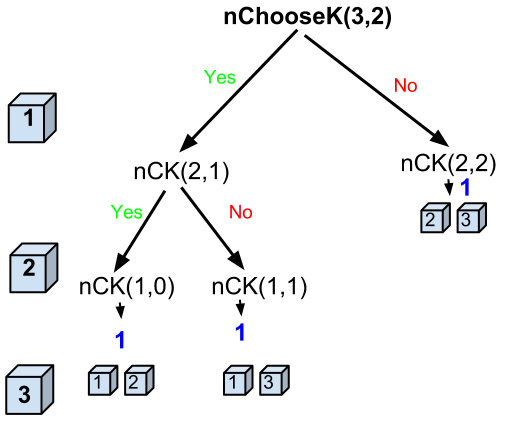
\includegraphics[scale=0.5]{nChooseK.png}
\end{frame}

\subsection{Multiple Recursion}
\begin{frame}[fragile]{Multiple Recursion}
  This problem is modified from lab 8, Exercise 4.

  Consider an insect in an $M$ by $N$ grid. The insect starts at the left
  corner, $(0,0)$, and wants to end up at the bottom right corner,
  $(M-1,N-1)$.

  Every minute, the insect is capable of moving right or down \emph{any
  number of squares between $1$ and $l$}. Write a function that determines
  the number of ways the insect can go from start to finish if we regard
  each minute as a distinct state.

  \begin{lstlisting}
def countpaths(M,N,l):
  \end{lstlisting}

  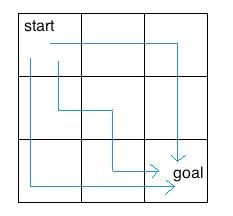
\includegraphics[scale=0.5]{insect.jpeg}
\end{frame}

\begin{frame}[fragile]{Multiple Recursion}
  Below is an example of calling countpaths(3,2,2)

  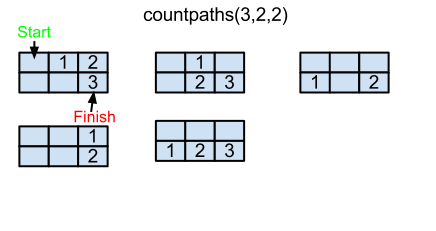
\includegraphics[scale=0.5]{countpaths.png}
\end{frame}

\begin{frame}[fragile]{Multiple Recursion}

  \begin{lstlisting}
def countpaths(M,N,l):
    return helper(M,N,l,l,0,0)

def helper(M,N,l,steps,x,y):
    if x == M - 1 and y == N - 1:
        return 1
    elif x > M-1 or y > M - 1:
        return 0
    else:
        if steps == 0:
            return 0
        else:
            return helper(M,N,l,steps-1,x,y) +
                helper(M,N,l,l,x+steps,y) +
                helper(M,N,l,l,x,y+steps)
  \end{lstlisting}
\end{frame}

% Order of Growth %
% ------------------------------------------------------------------------ %
\section{Order of Growth}
\subsection{Order of Growth}
\begin{frame}[fragile]{Order of Growth}
  What is the order of growth for the following function?

  \begin{lstlisting}
def fib1(n):
    if n == 1:
        return 1
    elif n == 2:
        return 1
    else:
        return fib1(n-1)+fib1(n-2)
  \end{lstlisting}

  \begin{enumerate}
    \item
      $O(1)$
    \item
      $O(\text{log}n)$
    \item
      $O(n)$
    \item
      $O(n^2)$
    \item
      \alert<2>{$O(2^n)$}
  \end{enumerate}
\end{frame}

\begin{frame}[fragile]{Order of Growth}
  What is the order of growth for the following function?

  \begin{lstlisting}
def fib2(n):
    ls = [1,1]
    for i in range(2,n):
        ls.append(ls[-1]+ls[-2])
    return ls[-1]
  \end{lstlisting}

  \begin{enumerate}
    \item
      $O(1)$
    \item
      $O(\text{log}n)$
    \item
      \alert<2>{$O(n)$}
    \item
      $O(n^2)$
    \item
      $O(2^n)$
  \end{enumerate}
\end{frame}

\begin{frame}[fragile]{Order of Growth}
  What is the order of growth for the following function?

  \begin{lstlisting}
def foo(n):
    if n <= 1:
        return 0
    else:
        return 1 + foo(n/2)
  \end{lstlisting}

  \begin{enumerate}
    \item
      $O(1)$
    \item
      \alert<2>{$O(\text{log}n)$}
    \item
      $O(n)$
    \item
      $O(n^2)$
    \item
      $O(2^n)$
  \end{enumerate}
\end{frame}

% Classes %
% ------------------------------------------------------------------------ %
\section{Classes}
\subsection{Classes}

\begin{frame}[fragile]{Classes}
  Convert the following below-the-line implementation of a class
  representing a point on the cartesian plane to a Python 3 class:

  \begin{lstlisting}[basicstyle=\small]
from math import *
def make_point(x, y):
    def point(op, *opnds):
        nonlocal x, y
        if op == 'distance_from_origin' and len(opnds) == 0:
            return sqrt(pow(x, 2) + pow(y, 2))
        elif op = 'distance_from_point' and len(opnds) == 1:
            return sqrt(pow(x - opnds[0]('x'), 2)
                + pow(y - opnds[0]('y'), 2))
        elif op = 'x' and len(opnds) == 0:
            return x
        elif op = 'y' and len(opnds) == 0:
            return y
        else:
            raise ValueError()
    return point
  \end{lstlisting}
\end{frame}

\begin{frame}[fragile]{Classes}
  Solution

  \begin{lstlisting}[basicstyle=\small]
from math import *
class Point:
    def __init__(self, x, y):
        self.x, self.y = x, y

    def distance_from_origin(self):
        return sqrt(pow(self.x, 2) + pow(self.y, 2))

    def distance_from_point(self, p):
        return sqrt(pow(self.x-p.x, 2) + pow(self.y-p.y, 2))
  \end{lstlisting}
\end{frame}

\subsection{Identifying Parts of Classes}
\begin{frame}[fragile]{Identifying Parts of Classes}
  Consider the following class:

  \begin{lstlisting}
class Foo:
    x = 3
    def __init__(self, var):
        self.y = var

    def bar(self, z):
        Foo.x = Foo.x + 1
        return self.y + z

f = Foo()
  \end{lstlisting}

  Identify variables that reference
  \begin{enumerate}
    \item
      A class: \uncover<2->{\alert<2>{Foo}}
    \item
      An instance variable: \uncover<3->{\alert<3>{y}}
    \item
      A static variable: \uncover<4->{\alert<4>{x}}
    \item
      A method: \uncover<5->{\alert<5>{bar, \_\_init\_\_}}
    \item
      A parameter: \uncover<6->{\alert<6>{self, var, z}}
    \item
      An object: \uncover<7->{\alert<7>{f}}
  \end{enumerate}

\end{frame}

\subsection{Facepalm}
\begin{frame}[fragile]{Classes}
  It is 2001 and you are a college student at Cal. You decide to create {\sc
  Facepalm}, an application for the Palm Pilot that maintains information
  about different people in your address book. {\sc Facepalm} will have a
  {\em profile} for each person. You decide to write a class called {\tt
  Profile} that simulates a {\sc Facepalm} profile. It stores a person's
  name, the person's institution, and a list of profiles of the person's
  friends. It also has the following methods:

  \begin{enumerate}
    \item
      \textcolor{blue}{\tt add\_friend(profile)} adds the given profile to
      the list of profiles of friends, if the profile is not already
      present.
    \item
      \textcolor{blue}{\tt get\_name()} returns the person's name.
    \item
      \textcolor{blue}{\tt get\_inst()} returns the person's institution.
  \end{enumerate}

  Write the definition of the {\tt Profile} class as specified above. We
  have given you a template.

  \begin{lstlisting}
class Profile:
    def __init__(self, name, inst):
        pass
  \end{lstlisting}
\end{frame}

\begin{frame}[fragile]{Classes}
  Solution:
  \begin{lstlisting}[basicstyle=\small]
class Profile:
    def __init__(self, name, inst):
        self.name = name
        self.inst = inst
        self.friends = []

    def add_friend(self, profile):
        if profile not in self.friends:
            self.friends.append(profile)

    def get_name(self):
        return self.name

    def get_inst(self):
        return self.inst
  \end{lstlisting}
\end{frame}

\begin{frame}[fragile]{Dictionaries}
  You now want to give a user a sense of the geographical distribution of
  their friends. To achieve that, you provide a method {\tt
  friends\_in\_inst}, which returns a dictionary that maps an institution to
  a list of the profiles of all the friends at that institution. Write the
  definition of {\tt{friends\_in\_inst}}.

  \begin{lstlisting}
class Profile:
    ...
    def friends_in_inst(self):
        ''' FILL ME IN '''
        pass
  \end{lstlisting}
\end{frame}


\begin{frame}[fragile]{Dictionaries}
  Solution:

  \begin{lstlisting}
class Profile:
    ...
    def friends_in_inst(self):
        result = {}
        for friend_profile in self.friends:
            inst = friend_profile.inst
            if inst in result:
                result[inst].append(friend_profile)
            else:
                result[inst] = [friend_profile]
        return result
  \end{lstlisting}
\end{frame}

\begin{frame}[fragile]{Inheritance}
  You are not earning too much money from the application.  In an attempt to
  get some revenue, you decide that profiles will be "restricted" by
  default: when restricted, users are only allowed to add 100 friends,
  beyond which they will not be allowed to add more friends.  You then offer
  "paid" profiles that lift this restriction.

  \begin{enumerate}
    \item
      Modify the definition of {\tt add\_friend} in the class {\tt Profile}
      that implements the restriction.
    \item
      Define another class called {\tt Paid\_profile} that mimics the {\tt
      Profile} class, except in the behavior of the {\tt add\_friend}
      method. ({\em Hint}: You should not have to rewrite a lot of {\tt
      Profile}.)
  \end{enumerate}
\end{frame}


\begin{frame}[fragile]{Inheritance}
  Solution:
  \begin{lstlisting}
class Profile:
    ...
    def add_friend(self, profile):
        if profile not in self.friends:
            if len(self.friends) < 100:
                self.friends.append(profile)
            else:
                print "Cannot add more than 100
                       friends. Please upgrade."

class Paid_profile(Profile):
    def add_friend(self, profile):
        if profile not in self.friends:
            self.friends.append(profile)
  \end{lstlisting}
\end{frame}


\begin{frame}[fragile]{Epilogue}
  The application, unfortunately, dies out because you have not had a chance
  to move it to other platforms. However, in 2003, a Harvard student named
  Mark Zuckerberg comes up with a suspiciously similar idea...
\end{frame}


% Mutable Data %
% ------------------------------------------------------------------------ %
\section{Mutable Data}
\subsection{List Mutation}

\begin{frame}[fragile]{Destructive map}
  Write a destructive method {\tt d\_map()} that takes in a function {\tt f}
  and a list {\tt l} and changes the list so that each element {\tt e} is
  changed to {\tt f(e)}. For example,

  \begin{lstlisting}
>>> l = [1, 2, 3]
>>> d_map(lambda x: x + 1, l)
>>> l
[2, 3, 4]
  \end{lstlisting}
\end{frame}

\begin{frame}[fragile]{Destructive map}
  Solution

  \begin{lstlisting}
def d_map(f, l):
    for i in range(len(l)):
        l[i] = f(l[i])
  \end{lstlisting}

\end{frame}

\section{Memoization}
\subsection{Memoization}

\begin{frame}[fragile]{Memoization}
  Consider the mapping of the numbers $1, 2, \dots, 26$ to the letters where
  $1$ maps to {\tt A}, $2$ maps to {\tt B}, and so on.

  Given a string of numbers, how many ways are there to insert spaces such
  that all the numbers correspond to valid letters (i.e., are in $\{1, 2,
  \dots, 26\}$)? For example, for the string {\tt '1012'}, there are two
  ways:

  \begin{itemize}
    \item
      10, 1, 2
    \item
      10, 12
  \end{itemize}

  The splitting into {\tt 1, 0, 12} is not valid because {\tt 0} does not
  correspond to a letter. Also, the splitting into {\tt 1, 01, 2} is not
  valid because {\tt 01} does not correspond to a letter.
\end{frame}

\begin{frame}[fragile]{Memoization}
  The following function definition is a recursive solution. This function
  is very inefficient. Write a version that uses memoization to reduce the
  number of recursive calls.

  \begin{lstlisting}
def num_of_splits(s):
    if len(s) == 0:
        return 1
    else:
        return (check1(s) * num_of_splits(s[1:]))
            + (check2(s) * num_of_splits(s[2:]))

def check1(s):
    return s[0] in '123456789'

def check2(s):
    if len(s) > 1:
        if s[0] == '1':
            return s[1] in '0123456789'
        elif s[0] == '2':
            return s[1] in '0123456'
    return False
  \end{lstlisting}
\end{frame}

\begin{frame}[fragile]{Memoization}
  Solution:

  \begin{lstlisting}
def num_of_splits2(s):
    m = {}
    def helper(s):
        if s in m:
            return m[s]
        elif len(s) == 0:
            return 1
        else:
            m[s] = (check1(s) * helper(s[1:])) +
                (check2(s) * helper(s[2:]))
            return m[s]
    return helper(s)
  \end{lstlisting}
\end{frame}



\end{document}
